%% Springer Nature journal format — sn-mathphys-num (numbered references)
\documentclass[pdflatex,sn-mathphys-num]{sn-jnl}

\usepackage{graphicx}
\usepackage{multirow}
\usepackage{amsmath,amssymb,amsfonts}
\usepackage{amsthm}
\usepackage[title]{appendix}
\usepackage{xcolor}
\usepackage{textcomp}
\usepackage{booktabs}
\usepackage{url}
\usepackage{enumitem}
\setlist[itemize]{label=\textbullet,leftmargin=1.5em,itemsep=2pt,topsep=3pt}
\usepackage{hyperref}
\hypersetup{colorlinks=true,linkcolor=blue,citecolor=blue,urlcolor=blue}
\graphicspath{{figures/}{../figures/}}

\theoremstyle{thmstyleone}
\newtheorem{theorem}{Theorem}
\theoremstyle{thmstylethree}
\newtheorem{definition}{Definition}
\raggedbottom

\renewcommand{\orcidlogo}{
\includegraphics[width=8pt]{Orcidlogo.pdf}}
\renewcommand{\orcid}[1]{\unskip\,\href{https://orcid.org/#1}{\orcidlogo}}

\begin{document}

\title[From CLV Ranking to Uplift-Aware Targeting]{From Customer Lifetime Value Ranking to
Uplift-Aware Targeting: Cross-Context Evidence from Online Retail, Grocery, and Supermarket
Campaign Data}

\author[1]{\fnm{Vu Minh Anh} \sur{Nguyen}}\email{anhnvmse203412@fpt.edu.vn}
\author*[1]{\fnm{Linh Hoang} \sur{Nguyen}}\email{linhnh67@fpt.edu.vn}

\affil*[1]{%
  \orgdiv{Department of Information Technology},
  \orgname{FPT University},
  \orgaddress{\city{Ho Chi Minh City}, \country{Vietnam}}}

\abstract{Customer lifetime value (CLV) models identify \emph{who is valuable}; uplift models
identify \emph{who is responsive} to marketing. These objectives are seldom studied together or
across heterogeneous retail contexts. This work connects explainable CLV ranking with uplift-aware
targeting on three datasets spanning UK e-commerce, US grocery, and a randomised supermarket SMS
campaign. First, under a walk-forward protocol aligned with prior work, a Hurdle--Semantic CLV
framework remains competitive across the two CLV contexts, though the dominant mechanism shifts --
e-commerce is incidence-dominated, grocery is sequence-dominated -- and a leave-one-group-out ablation shows
sequence features significantly help grocery while semantic profiles mainly aid interpretation.
Second, on the campaign data, ranking by predicted \emph{response} is \emph{worse than random} for
incremental targeting, whereas uplift learners recover persuadable customers. Third, value and
persuadability select almost disjoint customers (top-decile overlap $0.7\%$), and a
\emph{value-adjusted uplift} score ($\hat\tau_i\cdot\hat V_i$) achieves the highest point estimate of profit
under tight budgets, although these monetary differences do not reach
statistical significance. In short: CLV identifies who is valuable, uplift identifies who is
responsive, and value-adjusted uplift identifies who is worth targeting.}

\keywords{customer lifetime value, uplift modelling, explainability, conformal prediction,
cross-context generalisation, campaign targeting}

\maketitle

\section{Introduction}\label{sec:intro}
Customer lifetime value (CLV) prediction and uplift modelling are two mature but largely separate
strands of marketing analytics. CLV studies rank customers by expected future value and direct
retention budgets towards the high-value tail. Uplift studies, by contrast, estimate the
\emph{incremental} effect of a marketing action and direct campaign budgets towards customers
whose behaviour actually changes when treated. The two objectives can disagree sharply: a loyal
high-value shopper who would return anyway yields little incremental revenue if targeted, whereas a
mid-value customer who only re-purchases when prompted -- the ``persuadable'' -- is invisible to a
value model but is exactly whom a campaign should reach.

Despite the practical importance of this distinction, three gaps remain. (i) CLV and uplift are
rarely evaluated within a single, comparable pipeline. (ii) CLV frameworks are seldom stress-tested
across structurally different retail contexts, so claims of generality are largely untested.
(iii) Targeting studies frequently optimise either value or response in isolation, leaving the
combined ``who is both valuable and persuadable'' question unanswered. These gaps are addressed with
an explainable, uncertainty-aware framework evaluated across three datasets, and with an explicit
\emph{value-adjusted uplift} targeting rule.

The study is organised around four research questions:
\begin{itemize}
  \item[\textbf{RQ1}] How robust is the explainable Hurdle--Semantic CLV framework when
  re-estimated across UK online retail and US grocery contexts?
  \item[\textbf{RQ2}] Do semantic product profiles and behavioural sequence features provide
  incremental value beyond RFM for CLV ranking, calibration, and interpretation?
  \item[\textbf{RQ3}] On campaign data with treatment/control labels, does uplift-aware targeting
  outperform CLV-only, RFM-only, and response-model targeting?
  \item[\textbf{RQ4}] Can combining predicted customer value with uplift scores improve simulated
  campaign efficiency, and what transferable design principles follow for budget-constrained
  retail campaigns?
\end{itemize}

\noindent\textbf{Contributions.} (1) A cross-context evaluation showing the Hurdle--Semantic
framework stays competitive, with a leading mechanism that depends on context zero-inflation
(RQ1). (2) A leave-one-group-out ablation isolating where each feature group helps -- sequence in
grocery, semantic mainly for interpretation -- with SHAP and conformal analyses (RQ2). (3) Evidence
that response-based targeting is \emph{worse than random} for incremental campaigns (RQ3). (4) A
value-adjusted uplift policy with a profit simulation and an honest account of when it helps (RQ4).

\section{Related Work}\label{sec:related}
\subsection{CLV prediction and explainability}
Customer-base analysis has a long lineage of probability models that estimate future value from
RFM summaries \citep{fader2005rfm,gupta2006modeling}. Retail CLV is typically zero-inflated
and heavy-tailed, which motivates two-part Hurdle models and zero-inflated lognormal formulations
that separate purchase incidence from spend magnitude \citep{cragg1971hurdle,wang2019deep}. Beyond RFM, sequence and temporal features \citep{bauer2021improved} and learned product
embeddings \citep{chamberlain2017customer} enrich tabular CLV models, commonly trained with
gradient boosting \citep{ke2017lightgbm}. For decision support, post-hoc attribution \citep{lundberg2017unified} and calibrated
uncertainty are increasingly expected; conformalized quantile regression \citep{romano2019cqr}
yields intervals with valid marginal coverage under heteroscedasticity.

\subsection{Uplift modelling and heterogeneous treatment effects}
Uplift (true-lift) modelling estimates the incremental impact of a treatment rather than the
response level \citep{gutierrez2017uplift}. Meta-learners
(S-, T-, and X-Learners) and causal forests learn heterogeneous treatment effects with flexible
base learners \citep{kunzel2019metalearners,wager2018causalforest}.
Closest in motivation, the analysis of \citep{ascarza2018retention} shows that targeting the
highest-risk (or highest-propensity) customers can be ineffective because they would act anyway --
the empirical core of the ``response $\neq$ persuadable'' finding.

\subsection{Profit-driven and value-based targeting}
A separate strand argues that targeting should optimise profit, not response: profit-driven churn
and campaign models \citep{verbeke2012new,lemmens2020managing,gubela2024multiple}, and policy
evaluation that ranks targeting rules by incremental value \citep{hitsch2024heterogeneous}. This work bridges these strands by \emph{combining} an explainable CLV
value estimate with an uplift estimate into a single value-adjusted policy, and by evaluating that
policy across structurally different retail contexts. Unlike that line of work -- typically single-domain, black-box, and reporting point performance -- the present study adds cross-context validation, SHAP-based interpretation, honest significance testing, and an explicit value-versus-persuadability overlap analysis. Methodologically, the contribution is not a new estimator but a value-adjusted \emph{policy} ($\hat\tau_i\hat V_i$) evaluated head-to-head against CLV-only and uplift-only policies, with an overlap analysis that quantifies how differently they select customers.


\section{Data and Problem Setup}\label{sec:data}
Three datasets with deliberately separated roles are used. \textbf{Online Retail II} (UK
e-commerce) is the baseline CLV context, reused read-only from prior work. \textbf{Dunnhumby
Complete Journey} (US grocery; $2{,}500$ households, $102$ weeks, $2.6$M lines) is an \emph{external}
CLV validation context. \textbf{X5 RetailHero} provides a randomised SMS campaign with
treatment/control labels for $200{,}039$ clients and $45.7$M pre-communication purchase lines.

To keep the causal claim clean, coupon redemption in Dunnhumby -- a \emph{post-campaign outcome},
not a clean assignment -- is \emph{not} used as a treatment. Uplift estimation is restricted to
the randomised X5 design (balanced, treatment ratio $0.500$; raw uplift $+3.32$pp, $95\%$ CI
$[2.90,3.75]$); Dunnhumby serves only CLV validation. The CLV target over a horizon is
$Y_i=\sum_{t}\text{Revenue}_{i,t}$. The two CLV contexts differ sharply: Online Retail II has a
$\sim50\%$ zero rate and non-zero skewness $\approx16.7$ (sparse, heavy-tailed), whereas Dunnhumby
has a $\sim7\%$ zero rate and skewness $\approx2.5$ (dense, light-tailed) -- a structural contrast
that makes RQ1 a genuine robustness test.

\section{Methodology}\label{sec:method}
\subsection{Module A --- Hurdle CLV ranking}
Value is decomposed into incidence and magnitude,
\begin{equation}
\widehat{CLV}_i = p_i \cdot m_i, \quad p_i = P(Y_i>0\mid X_i), \quad m_i = \mathbb{E}[Y_i\mid Y_i>0, X_i],
\end{equation}
where stage~1 is a gradient-boosted classifier and stage~2 a gradient-boosted regressor on
$\log Y_i$ restricted to positive customers. A lognormal bias correction is applied,
$m_i=\exp(\hat\mu_i+\hat\sigma^2/2)$, with $\hat\sigma^2$ the residual variance of stage~2. The
decomposition is attractive when the target is a mixture of structural zeros and a heavy-tailed
positive part.

\subsection{Module B --- Semantic product profiling}
A basket-level product co-occurrence matrix is transformed by positive point-wise mutual
information and factorised by truncated SVD into $32$-dimensional product embeddings. Each
customer's taste vector is the revenue-weighted mean of the embeddings of the products they
bought, computed over the full observation window and the last $90$ days to capture taste drift.

\subsection{Module C --- Uplift learners}
With treatment $T_i\in\{0,1\}$ and outcome $Y_i$, the uplift is
$\tau_i=E[Y_i(1)-Y_i(0)\mid X_i]$. It is estimated with an S-Learner (a single model with treatment
as a feature), a T-Learner (separate treated/control models), an X-Learner (a two-stage
meta-learner that imputes individual effects and regresses on them), and a class-transformation
model. These are compared with a response model (which ranks by $P(Y_i=1)$ ignoring treatment) and a
random baseline.

\subsection{Module D --- Value-adjusted uplift (central contribution)}
The central targeting rule, and the main contribution of this work, scores customers by
\begin{equation}
\text{Score}^{\text{VU}}_i = \hat\tau_i \cdot \hat V_i,
\end{equation}
where $\hat V_i$ is a value proxy derived from historical spend. Notably, $\hat V_i$ is a
\emph{proxy}, not an observed future CLV, and results are reported accordingly.

\subsection{Evaluation protocol}\label{sec:protocol}
\paragraph{CLV: walk-forward (temporal).} CLV is a forecasting task, so a random split would leak
future structure. CLV is therefore evaluated with a \emph{walk-forward} design. For Online Retail
II, the Phase~1 walk-forward windows are reused (anchored 1~Dec~2009; benchmark windows W1--W3, with
W4--W5 as extended robustness), using the same RFM and behavioural features and the same VIP label. This makes the Phase~2 numbers directly comparable to, and consistent with, Phase~1. For Dunnhumby,
four week-level windows are built (observation$\to$prediction: 26$\to$8, 39$\to$13, 52$\to$13,
78$\to$13 weeks). Within each window a stratified $80/20$ split on the top-decile VIP indicator (seed $42$) is used;
Normalized Gini (NG), Revenue Capture@$10\%$ (RC@10), Precision@$10\%$, Spearman, and decile
calibration are reported as the \emph{mean $\pm$ std across windows}.
\paragraph{Uplift: randomised cross-section.} The X5 campaign is a cross-sectional randomised
design, so a $70/30$ split stratified on the joint of treatment and outcome is used, reporting
Qini AUC, AUUC, and uplift@$K$. Because treatment is randomised, any top-$K$ set contains both
treated and control customers, so incremental conversions and revenue are the difference in group
means scaled by the number targeted. Uncertainty is quantified with the percentile bootstrap
($B=1000$ for CLV, $B=400$ for uplift), reporting paired differences with $95\%$ confidence
intervals.

\subsection{Implementation details}\label{sec:impl}
For reproducibility the following choices are fixed. \emph{Preprocessing.} Online Retail~II drops
cancelled invoices (invoice codes starting with \texttt{C}), non-positive quantity or price, and rows
with a missing customer identifier; revenue is quantity$\times$price, giving $805{,}549$ transactions
for $5{,}038$ customers (matching Phase~1). Dunnhumby uses all $2{,}500$ households with net sales
value as revenue; coupon and promotion variables are \emph{not} used as a treatment. X5 features are
aggregated strictly from pre-communication purchases, and the outcome is the binary purchase-response
label supplied by the RetailHero benchmark; no post-campaign revenue is released, hence the pre-period
value proxy. \emph{Models.} All gradient-boosted stages use LightGBM: the Hurdle classifier ($400$
trees, learning rate $0.03$) and regressor ($500$ trees, $0.03$); the uplift base learner is a
LightGBM classifier ($300$ trees, $0.05$, $31$ leaves, subsample and colsample $0.8$, seed $42$).
The S-, T-, and class-transformation learners use \texttt{scikit-uplift}; the class-transformation
target is $z_i=Y_iT_i+(1-Y_i)(1-T_i)$ at propensity $\tfrac12$, so $\hat\tau_i=2\hat P(z_i{=}1)-1$,
and the X-Learner is implemented directly with LightGBM regressors averaged at propensity $0.5$.
Qini AUC, AUUC, and uplift@$K$ use the \texttt{scikit-uplift} implementations. \emph{Explainability
and uncertainty.} SHAP uses \textsc{TreeExplainer} on the Stage-2 regressor evaluated on the test
fold. CQR is split-conformal: an $80/20$ train/test split, with the training fold further split
$50/50$ into proper-training and calibration; LightGBM quantile regressors at levels $\alpha/2$ and
$1-\alpha/2$ are conformalised by the calibration residual quantile $\hat q$, and empirical coverage
is measured on the test fold at nominal $90\%$ and $80\%$.

\section{Results and Analysis}\label{sec:results}

\begin{table}[t]\centering
\caption{Walk-forward CLV benchmark. NG and RC@10 are mean $\pm$ std across temporal windows (Online Retail II on the Phase~1 windows W1--W3, Dunnhumby on D1--D4); Precision@10 is the across-window mean. Results are temporally valid and lie in the same range as the Phase~1 walk-forward benchmark (NG~$\approx$~0.83); small differences follow from the feature set and the window subset.}\label{tab:clvwf}
\begin{tabular}{lrrrr}
\hline
context & model & NG & RC@10 & Prec@10 \\
\hline
Online Retail II (W1-W3) & Hurdle & 0.825 $\pm$ 0.050 & 59.037 $\pm$ 9.466 & 0.577 \\
Online Retail II (W1-W3) & Monetary & 0.822 $\pm$ 0.058 & 60.017 $\pm$ 8.404 & 0.586 \\
Online Retail II (W1-W3) & RandomForest & 0.805 $\pm$ 0.043 & 56.883 $\pm$ 7.203 & 0.558 \\
Online Retail II (W1-W3) & Ridge & 0.805 $\pm$ 0.038 & 56.193 $\pm$ 8.234 & 0.547 \\
Online Retail II (W1-W3) & XGBoost & 0.802 $\pm$ 0.044 & 56.807 $\pm$ 8.818 & 0.540 \\
Online Retail II (W1-W3) & LightGBM & 0.799 $\pm$ 0.052 & 57.170 $\pm$ 9.850 & 0.547 \\
Dunnhumby (D1-D4) & RandomForest & 0.862 $\pm$ 0.012 & 34.297 $\pm$ 0.623 & 0.723 \\
Dunnhumby (D1-D4) & Ridge & 0.858 $\pm$ 0.009 & 34.280 $\pm$ 0.452 & 0.703 \\
Dunnhumby (D1-D4) & Hurdle & 0.855 $\pm$ 0.014 & 34.280 $\pm$ 0.457 & 0.714 \\
Dunnhumby (D1-D4) & XGBoost & 0.854 $\pm$ 0.014 & 34.235 $\pm$ 0.923 & 0.738 \\
Dunnhumby (D1-D4) & LightGBM & 0.849 $\pm$ 0.009 & 34.270 $\pm$ 0.778 & 0.723 \\
Dunnhumby (D1-D4) & Monetary & 0.825 $\pm$ 0.010 & 32.350 $\pm$ 0.712 & 0.658 \\
\hline
\end{tabular}
\end{table}

\begin{table}[t]\centering
\caption{X5 uplift model comparison (RQ3). The response model ranks below random.}\label{tab:uplift}
\begin{tabular}{lrrrr}
\hline
model & Qini\_AUC & AUUC & uplift@10 & uplift@20 \\
\hline
S-Learner & 0.014 & 0.020 & 0.112 & 0.077 \\
X-Learner & 0.012 & 0.018 & 0.104 & 0.072 \\
T-Learner & 0.010 & 0.015 & 0.087 & 0.069 \\
ClassTransform & 0.008 & 0.011 & 0.086 & 0.064 \\
Random & -0.002 & -0.004 & 0.026 & 0.029 \\
ResponseModel & -0.007 & -0.011 & 0.004 & 0.008 \\
\hline
\end{tabular}
\end{table}

\begin{table}[t]\centering
\caption{Targeting policy comparison on X5 (RQ4). The value proxy $\hat V_i$ is pre-period historical monetary spend (a gross-value proxy, not future CLV). Incremental conversions and incremental value are held-out treated-minus-control estimates within each selected top-$K$ set (Eq.~\ref{eq:profit}); the headline uses margin $m=1$, so profit $=$ (incr.\ value) $-$ contact cost with $c=100$ rubles per contact (value and profit in millions of rubles). Across a sensitivity sweep ($m\in\{0.1,0.2,0.3\}$, $c\in\{50,100,200\}$) value-adjusted uplift has the highest point-estimate profit in all nine settings.}\label{tab:policy}
\begin{tabular}{lrrrr}
\hline
policy & K & incr. conv. & incr. value (M) & profit (M) \\
\hline
Random & 10\% & 129.4 & 0.29 & -0.31 \\
Random & 20\% & 351.5 & 0.13 & -1.07 \\
RFM-only & 10\% & 52.0 & 0.11 & -0.49 \\
RFM-only & 20\% & 109.7 & 1.96 & 0.76 \\
Value-only(CLV proxy) & 10\% & 77.3 & -0.05 & -0.65 \\
Value-only(CLV proxy) & 20\% & 263.0 & 4.56 & 3.36 \\
Uplift-only(S-Learner) & 10\% & 670.4 & 1.09 & 0.49 \\
Uplift-only(S-Learner) & 20\% & 930.1 & 3.23 & 2.03 \\
Value-adjusted(uplift x value) & 10\% & 248.4 & 1.34 & 0.74 \\
Value-adjusted(uplift x value) & 20\% & 451.7 & 5.23 & 4.03 \\
\hline
\end{tabular}
\end{table}

\begin{table}[t]\centering
\caption{Significance of key claims ($\Delta$NG with walk-forward paired $t$-tests for CLV; bootstrap for the uplift Qini comparison). With only 3--4 windows, the CLV tests are robustness diagnostics rather than definitive inference. Only sequence-in-grocery and uplift-vs-response are significant.}\label{tab:robust}
\begin{tabular}{lrr}
\hline
claim & $\Delta$NG & $p$ \\
\hline
Hurdle $>$ Monetary (e-com, walk-fwd) & $+0.0030$ & $0.554$ \\
Hurdle vs RandomForest (grocery, walk-fwd) & $-0.0064$ & $0.063$ \\
extra features $>$ RFM (e-com) & $+0.0092$ & $0.1668$ \\
extra features $>$ RFM (grocery) & $+0.0444$ & $0.0021$ \\
semantic adds ranking (e-com) & $+0.0028$ & $0.5835$ \\
semantic adds ranking (grocery) & $+0.0011$ & $0.8373$ \\
sequence adds ranking (grocery) & $+0.0206$ & $0.0011$ \\
S-Learner $>$ Response (uplift Qini) & -- & $<0.001$ \\
\hline
\end{tabular}
\end{table}

\begin{table}[t]\centering
\caption{Leave-one-group-out ablation (Hurdle, walk-forward). dNG\_vs\_ALL $>$ 0 means dropping the group hurts; paired\_p is the paired t-test across windows.}\label{tab:ablation}
\begin{tabular}{lrrrrr}
\hline
context & variant & NG\_mean & NG\_std & dNG\_vs\_ALL & paired\_p \\
\hline
Online Retail II & ALL & 0.829 & 0.056 & 0.000 & -- \\
Online Retail II & ALL-behavioural & 0.829 & 0.052 & -0.000 & 0.954 \\
Online Retail II & ALL-semantic & 0.826 & 0.048 & 0.003 & 0.584 \\
Online Retail II & RFM-only & 0.820 & 0.063 & 0.009 & 0.167 \\
Dunnhumby & ALL & 0.856 & 0.015 & 0.000 & -- \\
Dunnhumby & ALL-behavioural & 0.856 & 0.015 & 0.000 & 0.088 \\
Dunnhumby & ALL-semantic & 0.855 & 0.016 & 0.001 & 0.837 \\
Dunnhumby & ALL-sequence & 0.836 & 0.017 & 0.021 & 0.001 \\
Dunnhumby & RFM-only & 0.812 & 0.013 & 0.044 & 0.002 \\
\hline
\end{tabular}
\end{table}

\begin{table}[t]\centering
\caption{Top-10\% targeting overlap between policies, defined as $|A_K\cap B_K|/K$ where $A_K,B_K$ are the top-$K$ customer sets selected by each policy. Value and Uplift select almost disjoint customers (0.007), evidencing that value $\neq$ persuadability.}\label{tab:overlap}
\begin{tabular}{lrr}
\hline
policy\_A & policy\_B & overlap \\
\hline
RFM & Value(CLV proxy) & 0.666 \\
RFM & Uplift(S-Learner) & 0.003 \\
RFM & Value-adjusted & 0.173 \\
Value(CLV proxy) & Uplift(S-Learner) & 0.007 \\
Value(CLV proxy) & Value-adjusted & 0.312 \\
Uplift(S-Learner) & Value-adjusted & 0.256 \\
\hline
\end{tabular}
\end{table}

\begin{table}[t]\centering
\caption{Conformalized quantile regression: empirical coverage and mean interval width per context. Coverage is close to nominal; grocery intervals are tighter, consistent with its lighter tail.}\label{tab:cqr}
\begin{tabular}{lrrr}
\hline
context & nominal\_coverage & empirical\_coverage & mean\_interval\_width \\
\hline
Online Retail II & 0.900 & 0.902 & 1,653 \\
Online Retail II & 0.800 & 0.793 & 1,315 \\
Dunnhumby & 0.900 & 0.890 & 707 \\
Dunnhumby & 0.800 & 0.778 & 515 \\
\hline
\end{tabular}
\end{table}


\subsection{Cross-context CLV ranking (RQ1, RQ2)}\label{sec:res_clv}
Table~\ref{tab:clvwf} reports the walk-forward CLV benchmark for both contexts as mean $\pm$ std
across temporal windows. On Online Retail II the Hurdle model attains the highest point estimate
(NG$=0.825\pm0.050$, RC@10$=59.0\%$) but is statistically indistinguishable from a strong
Monetary baseline (NG$=0.822$, paired $p=0.55$). On Dunnhumby it is again statistically tied with
regularised linear and tree models (NG$\approx0.855$, within one standard deviation), and is not
the top model. The framework thus remains \emph{competitive} across contexts rather than
dominant, while the leading mechanism shifts between them. These numbers are consistent with the
Phase~1 result (Hurdle NG$\approx0.83$), replacing an earlier inflated random-split estimate. The mechanism is visible in the
data structure: the $\sim50\%$ zero rate of e-commerce lets the Hurdle incidence stage carry
ranking information, whereas the $\sim7\%$ zero rate of grocery makes the problem
magnitude-dominated, where the two-part structure adds little.

For RQ2, a leave-one-group-out ablation is run under the walk-forward protocol
(Table~\ref{tab:ablation}, with paired tests in Table~\ref{tab:robust}). The honest picture is
nuanced. Adding all feature groups beats RFM significantly in grocery ($\Delta$NG$=+0.044$,
$p=0.002$, driven by sequence features) but \emph{not} significantly in e-commerce
($\Delta$NG$=+0.009$, $p=0.17$). Dropping the semantic group does \emph{not} significantly change
ranking in either context (paired $p=0.58$ and $0.84$), whereas dropping sequence significantly
hurts grocery ($p=0.001$). The claim is therefore limited to what the data support: sequence features are a
significant ranking driver in grocery, while semantic profiles are valuable for interpretation and
segmentation rather than as a stand-alone ranking booster -- consistent with the Phase~1 finding. The ALL row in Table~\ref{tab:ablation} differs slightly from the Hurdle row in Table~\ref{tab:clvwf} because the former uses the full feature-group set whereas the latter reports the base benchmark configuration.
Stage-2 SHAP attribution supports this reading (Fig.~\ref{fig:shap}): monetary value dominates
conditional spending in e-commerce, whereas recent-sequence spend dominates in grocery. Conformalized quantile regression
(Table~\ref{tab:cqr}) attains valid coverage in both contexts ($90\%\!\to\!90.2\%/89.0\%$), with
substantially tighter intervals in grocery, consistent with its lighter tail.

\begin{figure}[t]\centering
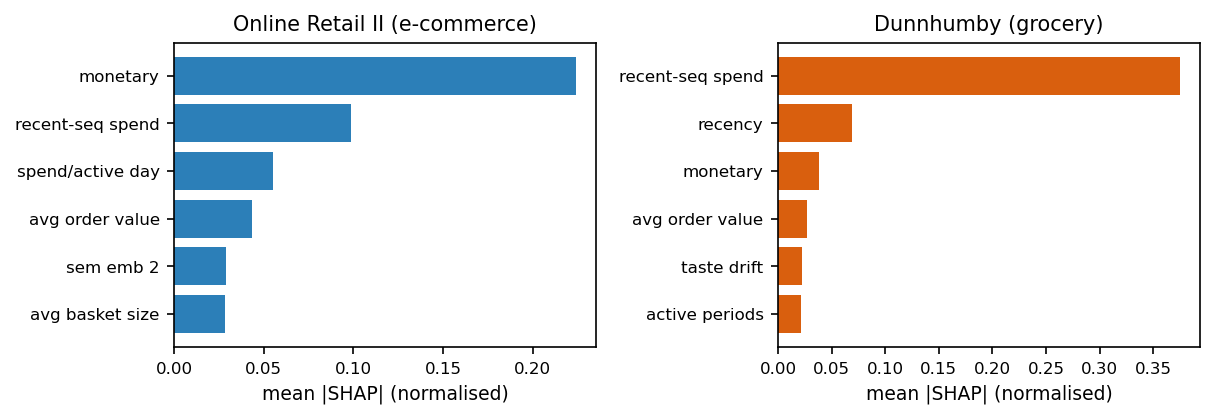
\includegraphics[width=0.95\columnwidth]{shap_crosscontext.png}
\caption{Stage-2 SHAP attribution (Hurdle model). In e-commerce, monetary value dominates conditional
spending; in grocery, recent-sequence spend is the leading driver. This supports the
context-dependent mechanism shift (RQ2).}\label{fig:shap}
\end{figure}

\subsection{Uplift-aware targeting (RQ3)}\label{sec:res_uplift}
The campaign is a balanced design: across all pre-communication covariates the standardised mean
difference between treated and control is below $0.01$, so group-mean
differences provide a low-bias estimate of incremental effects. Two evaluation regimes are kept
distinct: ranking quality (NG, RC@10, Qini) measures how well a score orders customers, whereas
the profit simulation evaluates the held-out economic outcome of acting on that score under a
budget.
Table~\ref{tab:uplift} delivers the central uplift result:
the response model ranks \emph{below random} (Qini $-0.007$; its bootstrap CI is entirely
negative, Table~\ref{tab:robust}), while uplift learners achieve positive Qini and reach
$\approx 11\%$ uplift in the top decile -- more than three times the average treatment effect.
Ranking by ``who is likely to buy'' actively selects sure buyers and therefore wastes budget;
ranking by estimated incremental effect recovers the persuadable segment. The paired bootstrap
difference between the best uplift learner and the response model is significant
($p<0.001$).

\subsection{Value-adjusted targeting and profit (RQ4)}\label{sec:res_policy}
A first finding is that value and persuadability identify different customers: the top-$10\%$ sets
chosen by a value (CLV-proxy) policy and an uplift policy overlap by only $0.007$
(Table~\ref{tab:overlap}). Value-adjusted uplift, by construction, blends the two (overlap $0.31$
with value and $0.26$ with uplift). Each policy scores every customer and selects the top-$K$ set
$A_K$; profit is then evaluated on the held-out RCT as
\begin{equation}
\widehat{\mathrm{Profit}}@K = m\,\widehat{\Delta V}_K - c\,|A_K|,\qquad
\widehat{\Delta V}_K = |A_K|\left(\overline{Y_i\hat V_i}\big|_{T=1,\,A_K} - \overline{Y_i\hat V_i}\big|_{T=0,\,A_K}\right),
\label{eq:profit}
\end{equation}
where $Y_i$ is the observed campaign outcome, $\hat V_i$ the pre-communication historical-monetary
value proxy (in rubles), $m$ a gross margin, and $c$ the per-contact cost. Crucially, the policy
score $\hat\tau_i\hat V_i$ is used \emph{only} to select $A_K$; profit is measured from the
treated-minus-control outcome difference \emph{within} $A_K$, so it is a held-out estimate and is
not mechanically implied by the score. Because X5 releases a binary purchase outcome but no
post-campaign revenue, $\widehat{\Delta V}_K$ is a value-weighted incremental-conversion estimate
(an expected value under the proxy $\hat V_i$) rather than observed revenue; profit is therefore an
expected, not observed, quantity and is reported with the hedge below. Table~\ref{tab:policy}
compares five policies by incremental conversions, incremental gross value, and profit (margin
$m=1$ in the headline). Targeting by value alone can \emph{lose} money at
small budgets, because the highest-value customers are disproportionately sure buyers with low
uplift; uplift-only targeting maximises the \emph{number} of incremental conversions; and
value-adjusted uplift achieves the highest point estimate of profit at tight budgets (Fig.~\ref{fig:profit})
by concentrating spend on high-value persuadables. This ranking is stable: in a sensitivity sweep
over $c\in\{50,100,200\}$ and $m\in\{0.1,0.2,0.3\}$, value-adjusted uplift remains the top policy by this point estimate across all nine settings.
Crucially, however, the bootstrap analysis (Table~\ref{tab:robust}) shows that while the
\emph{ranking}-level claims (uplift vs response; sequence in grocery) are significant, the
monetary profit differences between policies are directional rather than statistically
significant given test-set noise. This is stated explicitly rather than overclaimed.

\begin{figure}[t]\centering
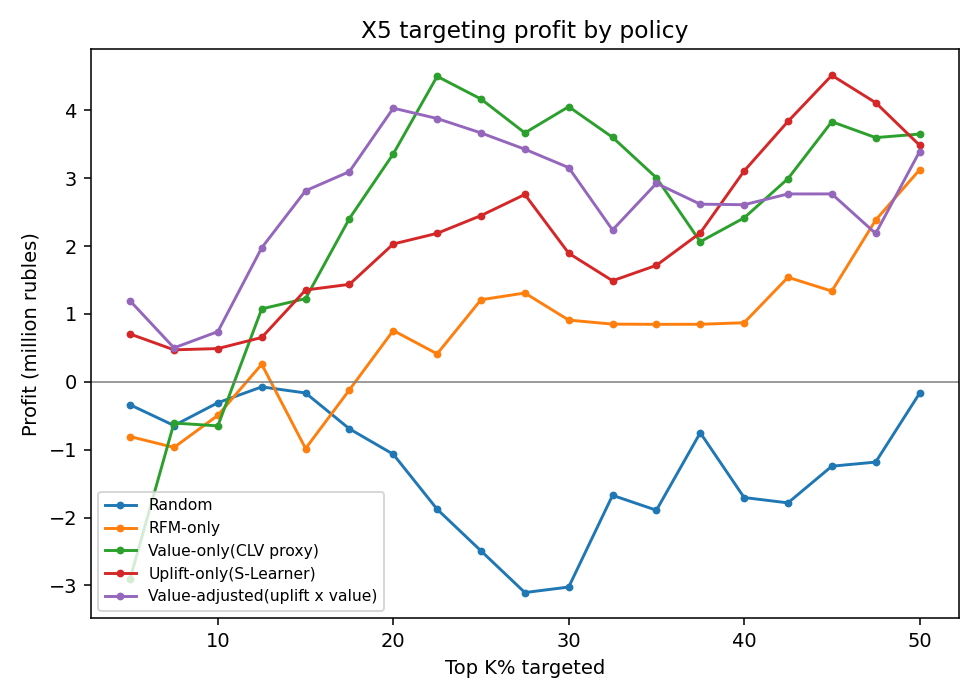
\includegraphics[width=0.78\textwidth]{x5_policy_profit.png}
\caption{Simulated targeting profit by policy and budget size (RQ4). Value-adjusted uplift achieves the
highest point-estimate profit at tight budgets; value-only targeting can be unprofitable.}\label{fig:profit}
\end{figure}

\section{Discussion}\label{sec:discussion}
\subsection{Why CLV and uplift disagree}
The disagreement is not marginal but near-total: the
value and uplift policies share only $0.7\%$ of their top decile (Table~\ref{tab:overlap}). The
mechanism is selection on different quantities -- value ranks on expected spend, which is highest
for already-loyal customers, whereas uplift ranks on the \emph{derivative} of spend with respect to
treatment, which is highest for marginal customers. This is the empirical counterpart of the
``retention futility'' argument \citep{ascarza2018retention}: the most valuable or most likely
customers are often the least movable, which is why value-only targeting can be unprofitable at
tight budgets. Value-adjusted uplift resolves the tension by multiplying the two signals,
recovering high-value \emph{persuadables}.
\subsection{Why the CLV mechanism shifts across contexts}
The two retail regimes differ in their
zero-inflation ($\sim50\%$ vs $\sim7\%$ zero rate): e-commerce is incidence-dominated, so the Hurdle
stage-1 carries information and the model is competitive; grocery is magnitude-dominated and
habitual, so recent-sequence behaviour is the significant driver and a two-part decomposition adds
little. The framework therefore \emph{transfers}, but which component does the work is
context-specific -- a caution against assuming a single architecture is universally best.
\subsection{Design principles}
Several principles follow, offered as transferable guidance rather
than numbers: targeting on value alone selects sure buyers and can lose money at tight budgets;
targeting on response alone can underperform random; value-adjusted uplift suits budget-constrained
settings; explainability clarifies \emph{why} a customer is selected; and calibrated uncertainty
matters when data are unstable. No direct numerical transfer to a specific market is claimed.

\subsection{Limitations}\label{sec:limits}
Several limitations bound these claims. The Dunnhumby CLV sample is modest ($\sim 2{,}500$
households), and the uplift evidence comes from a single SMS campaign in one market and period, so
external validity is untested. The X5 value $\hat V_i$ is pre-period historical spend, a proxy for
future value rather than an observed future CLV. Monetary profit differences between policies
are directional, not statistically significant, and absolute Qini values are modest because the raw
campaign signal is small ($\approx 3.3$ percentage points); the walk-forward CLV tests use only
3--4 windows, limiting paired-test power. Uplift is identified only on the randomised X5 design; no
causal claim is made on the observational CLV datasets.

\section{Conclusion and Future Work}\label{sec:conclusion}
Across three retail contexts, this work connects explainable CLV ranking with uplift-aware targeting. The
Hurdle--Semantic framework remains competitive across contexts, but the dominant mechanism is
context-dependent. The additional feature groups improve ranking mainly in grocery, driven by
sequence features, while semantic profiles aid interpretation more than aggregate ranking. On the
campaign data, response-based targeting is worse than random for incremental campaigns, and
value-adjusted uplift ranks first on point-estimate profit under tight budgets, though these
monetary differences are not statistically significant. CLV identifies who is valuable; uplift identifies who is responsive;
value-adjusted uplift identifies who is worth targeting. Future work includes jointly learned value-and-uplift objectives, multi-campaign and multi-market replication, and a field test of the value-adjusted policy under a real budget constraint.

\bibliography{references}

\end{document}
